\documentclass[12pt]{article}
\usepackage{amsmath, amssymb}
\usepackage{geometry}
\geometry{a4paper, margin=1in}
\usepackage{setspace}
\usepackage{lmodern}
\usepackage{graphicx}
\usepackage{titlesec}

% Formatting section headings
\titleformat{\section}[block]{\bfseries\Large}{\thesection.}{1em}{}
\titleformat{\subsection}[block]{\bfseries\large}{\thesubsection.}{1em}{}

\title{Question 3: Statistical Analysis of Test Grades}
\author{}
\date{}

\begin{document}
\maketitle
\onehalfspacing

\section*{Part 1: Frequency Distribution}
The histogram representing the test grades distribution is shown below:

\begin{center}
    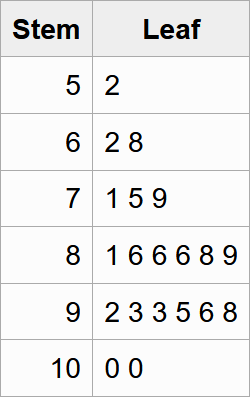
\includegraphics[width=0.3\textwidth]{Q3-P1-stemplot.png}
\end{center}

\textbf{Answer:} Histogram shown above.

\bigskip

\section*{Part 2: Descriptive Statistics}
Let the number of test scores be:
\[
n = 20.
\]
The data in ascending order:
\[
x_1 = 52, \quad x_2 = 62, \quad \dots, \quad x_n = 100.
\]

The range is:
\[
r = x_n - x_1 = 100 - 52 = 48.
\]

The mean is computed as:
\[
\bar{x} = \frac{1}{n} \sum_{i=1}^{n} x_i = 84.5.
\]

The standard deviation is given by:
\[
\sigma = \sqrt{\frac{1}{n} \sum_{i=1}^{n} x_i^2 - \bar{x}^2} = \frac{\sqrt{659}}{2} \approx 12.835.
\]

The indices for the quartiles are:
\[
\begin{alignedat}{2}
i_{Q_1} &= \frac{n}{4}+\frac{1}{2} &= 5.5, \\
i_{Q_2} &= \frac{n}{2}+\frac{1}{2} &= 10.5, \\
i_{Q_3} &= \frac{3}{4}n+\frac{1}{2} &= 15.5.
\end{alignedat}
\]

Calculating the quartiles:
\[
\begin{alignedat}{3}
Q_1 &= \frac{x_{\lceil i_{Q_1}-\frac{1}{2} \rceil} + x_{\lfloor i_{Q_1}+\frac{1}{2} \rfloor}}{2} &= \frac{x_5 + x_6}{2} &= 77, \\
Q_2 &= \frac{x_{\lceil i_{Q_2}-\frac{1}{2} \rceil} + x_{\lfloor i_{Q_2}+\frac{1}{2} \rfloor}}{2} &= \frac{x_{10} + x_{11}}{2} &= 87, \\
Q_3 &= \frac{x_{\lceil i_{Q_3}-\frac{1}{2} \rceil} + x_{\lfloor i_{Q_3}+\frac{1}{2} \rfloor}}{2} &= \frac{x_{15} + x_{16}}{2} &= 94.
\end{alignedat}
\]

The interquartile range (IQR) is:
\[
\mathrm{IQR} = Q_3 - Q_1 = 94 - 77 = 17.
\]

\textbf{Answer for Part 2:}
\[
Q_2 = 87, \quad \bar{x} = 84.5, \quad r = 48, \quad \sigma = \frac{\sqrt{659}}{2} \approx 12.835, \quad \mathrm{IQR} = 17.
\]

\bigskip

\section*{Part 3: Outlier Detection}
Using the outlier rule:
\[
Q_1 - 1.5 \times \mathrm{IQR} = 77 - 1.5 \times 17 = 51.5,
\]
\[
Q_3 + 1.5 \times \mathrm{IQR} = 94 + 1.5 \times 17 = 119.5.
\]

Since all values in the dataset satisfy:
\[
51.5 < x_1 < x_n < 119.5,
\]
there are no outliers.

\textbf{Answer:} No outliers.

\end{document}
